\documentclass[12pt, titlepage]{article}
\usepackage{graphicx}
\usepackage{float}
\restylefloat{table}

% Imported Packages
%------------------------------------------------------------------------------
\usepackage{amssymb}
\usepackage{amstext}
\usepackage{amsthm}
\usepackage{amsmath}
\usepackage{enumerate}
\usepackage{fancyhdr}
\usepackage[margin=1in]{geometry}
\usepackage{graphicx}
\usepackage{extarrows}
\usepackage{setspace}
%------------------------------------------------------------------------------

% Header and Footer
%------------------------------------------------------------------------------
\pagestyle{plain}  
\renewcommand\headrulewidth{0.4pt}                                      
\renewcommand\footrulewidth{0.4pt}                                    
%------------------------------------------------------------------------------

% Title Details
%------------------------------------------------------------------------------
\title{SE 3A04: Software Design III: Large System Design}
\author{Group \#5, Spaceship System Sabotage %Alliteration; always adored and absolutely amazing
		\\Pareek Ravi 001407109
		\\Pavle Arezina 001410366
		\\David Hobson 001412317
		\\Victoria Graff 001401451
		\\Julian Cassano 001406891
}
\date{\today}                               
%------------------------------------------------------------------------------

% Document
%------------------------------------------------------------------------------
\begin{document}
\maketitle	
\pagenumbering{arabic}
\tableofcontents
\listoftables
\listoffigures
\newpage

\section{Introduction}
\label{sec:introduction}
% Begin Section

This section should provide an brief overview of the entire document.

\subsection{Purpose}
\label{sub:purpose}
% Begin SubSection
\begin{enumerate}[a)]
	\item Delineate the purpose of the document
	\item Specify the intended audience for the document
\end{enumerate}
% End SubSection

\subsection{System Description}
\label{sub:system_description}
% Begin SubSection
\begin{enumerate}[a)]
	\item Give a brief description of the system. This could be a paragraph or two to give some context to this document.
\end{enumerate}
% End SubSection

\subsection{Overview}
\label{sub:overview}
% Begin SubSection
\begin{enumerate}[a)]
	\item Describe what the rest of the document contains 
	\item Explain how the document is organised
\end{enumerate}
% End SubSection

% End Section

\section{Use Case Diagram}
\label{sec:use_case_diagram}
% Begin Section
\begin{figure}[ht!]
\centering
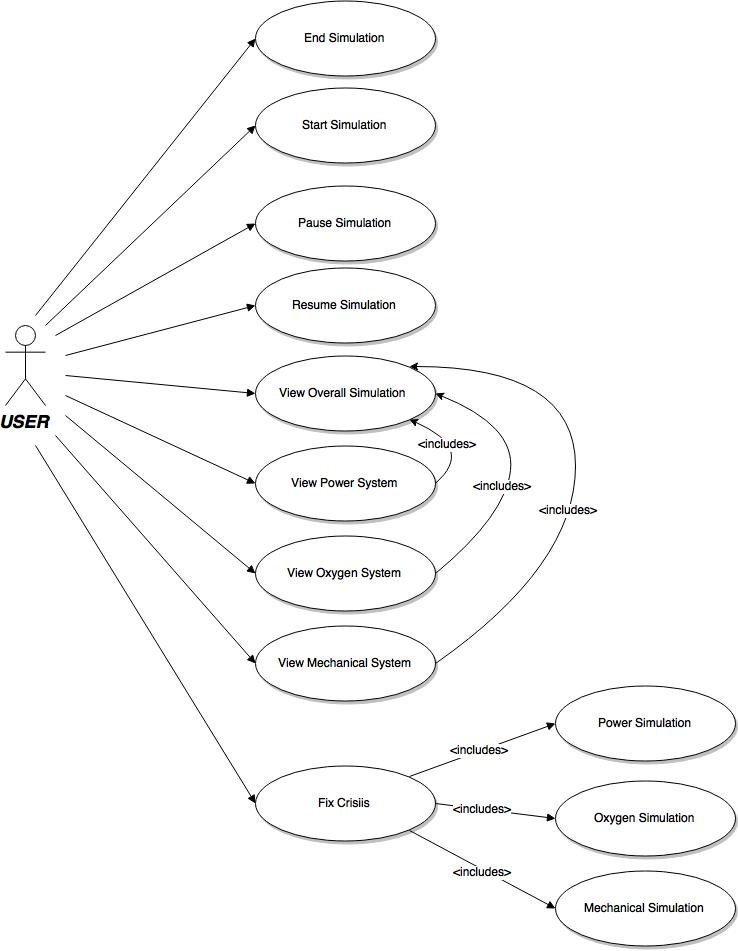
\includegraphics[width=120mm]{UseCase.jpg}
\caption{Use Case Diagram \label{usecase}}
\end{figure}
SHOW THE USE CASE DIAGRAM AND THEN EXPLAIN EACH SCENARIO
\begin{enumerate}[a)]
	\item End Simulation: The user is in a play session and intends to indefinitely stop the simulation and return to the main menu.
	\item Start Simulation: The user is in the main menu and intends to begin a play session.
	\item Pause Simulation: The user is in a play session and intends to stop the simulation but intends to resume at a later time.
	\item Resume Simulation: The user is in a paused play session and intends to resume and continue the simulation.
	\item View Overall System: The user is in a play session and intends to display the status of all the subsystems at once.
	\item View Power System: The user is in a play session and intends to include the status of the Power System in the displayed view.
	\item View Oxygen System: The user is in a play session and intends to include the status of the Oxygen System in the displayed view.
	\item View Mechanical System: The user is in a play session and intends to include the status of the Mechanical System in the displayed view.
	\item Fix Crisis: The user is in a play session and intends to resolve an event that is negatively affecting one of the subsystems.
	\item Fix Power: The user is in a fix crisis event and intends to resolve an event affecting the power system.
	\item Fix Oxygen: The user is in a fix crisis event and intends to resolve an event affecting the oxygen system.
	\item Fix Mechanical: The user is in a fix crisis event and intends to resolve an event affecting the mechanical system.
\end{enumerate}
% End Section

\section{Analysis Class Diagram}
\label{sec:analysis_class_diagram}
% Begin Section
DIAGRAM \\
See the CRC cards for explination for each class.
% End Section


\section{Architectural Design}
\label{sec:architectural_design}
% Begin Section
This section should provide an overview of the overall architectural design of your application. You overall architecture should show the division of the system into subsystems with high cohesion and low coupling.

\subsection{System Architecture}
\label{sub:system_architecture}
% Begin SubSection
\begin{enumerate}[a)]
	\item Identify and explain the overall architecture of your system
	\item Be sure to clearly state the name of the architecture
	\item Provide the reasoning and justification of the choice
	\item Provide a structural architecture diagram showing the relationship among the subsystems (if appropriate)
\end{enumerate}
% End SubSection

\subsection{Subsystems}
\label{sub:subsystems}
% Begin SubSection
\begin{enumerate}[a)]
	\item Provide a brief description of each subsystem. Be sure to document its purpose and relationship to other subsystems.
\end{enumerate}
% End SubSection

% End Section
	
\section{Class Responsibility Collaboration (CRC) Cards}
\label{sec:class_responsibility_collaboration_crc_cards}
% Begin Section
This section should contain all of your CRC cards.

\begin{enumerate}[a)]
	\item Provide a CRC Card for each identified class
	\item Please use the format outlined in tutorial, i.e., 
	\begin{table}[ht]
		\centering
		\begin{tabular}{|p{5cm}|p{5cm}|}
		\hline 
		 \multicolumn{2}{|l|}{\textbf{Class Name:}} \\
		\hline
		\textbf{Responsibility:} & \textbf{Collaborators:} \\
		\hline
		\vspace{1in} & \\
		\hline
		\end{tabular}
	\end{table}

%Start Screen	
	\begin{table}[H]
		\centering
		\begin{tabular}{|p{5cm}|p{5cm}|}
		\hline 
		 \multicolumn{2}{|l|}{\textbf{Class Name: Start Screen}} \\
		\hline
		\textbf{Responsibility:} & \textbf{Collaborators:} \\
		\hline
		 Receive request to display a prompt to start game& Menu Controller \\
		 Display screen message to user& \\
		 Respond to prompt being pressed by user& \\
		 Send request to Menu Controller to start game& Menu Controller \\
		\hline
		\end{tabular}
	\end{table}
	
%End Screen	
	\begin{table}[H]
		\centering
		\begin{tabular}{|p{5cm}|p{5cm}|}
		\hline 
		 \multicolumn{2}{|l|}{\textbf{Class Name: End Screen}} \\
		\hline
		\textbf{Responsibility:} & \textbf{Collaborators:} \\
		\hline
		 Receive request to display a prompt to end game& Menu Controller \\
		 Display screen message to user& \\
		 Respond to prompt being pressed by user& \\
		 Send request to Menu Controller to end game& Menu Controller \\
		\hline
		\end{tabular}
	\end{table}
	
%Pause Screen	
	\begin{table}[H]
		\centering
		\begin{tabular}{|p{5cm}|p{5cm}|}
		\hline 
		 \multicolumn{2}{|l|}{\textbf{Class Name: Pause Screen}} \\
		\hline
		\textbf{Responsibility:} & \textbf{Collaborators:} \\
		\hline
		 Receive request to display a prompt to pause game& Menu Controller \\
		 Display screen message to user& \\
		 Respond to prompt being pressed by user& \\
		 Send request to Menu Controller to pause and unpause game& Menu Controller \\
		\hline
		\end{tabular}
	\end{table}
	
%Success Screen	
	\begin{table}[H]
		\centering
		\begin{tabular}{|p{5cm}|p{5cm}|}
		\hline 
		 \multicolumn{2}{|l|}{\textbf{Class Name: Success Screen}} \\
		\hline
		\textbf{Responsibility:} & \textbf{Collaborators:} \\
		\hline
		 Receive request to display a screen message when game has been won& Menu Controller \\
		 Display screen message to user& \\
		\hline
		\end{tabular}
	\end{table}
	
%Failure Screen	
	\begin{table}[H]
		\centering
		\begin{tabular}{|p{5cm}|p{5cm}|}
		\hline 
		 \multicolumn{2}{|l|}{\textbf{Class Name: Failure Screen}} \\
		\hline
		\textbf{Responsibility:} & \textbf{Collaborators:} \\
		\hline
		 Receive request to display a screen message when game has been lost& Menu Controller \\
		 Display screen message to user& \\
		\hline
		\end{tabular}
	\end{table}	
	
	
\end{enumerate}
% End Section

\appendix
\section{Division of Labour}
\label{sec:division_of_labour}
% Begin Section
Include a Division of Labour sheet which indicates the contributions of each team member. This sheet must be signed by all team members.
% End Section
\begin{table}[h!]
\centering

\begin{tabular}{|c|c|c|}
\hline
{\bf Member} & {\bf Duties}&{\bf Signature}\\
\hline
{David Hobson} & { } & { }\\
{} & {}  & {}\\
\hline
{Pavle Arezina} & {} & {}\\
{} & {} & {}\\
\hline
{Pareek Ravi} & {} & {}\\
{} & {} & {}\\
\hline
{Victoria Graff} & {} & {}\\
{} & {} & {}\\
\hline
{Julian Cassano} & {} & {}\\
{} & {} & {}\\
\hline
\end{tabular}

\end{table}

\newpage
\section*{IMPORTANT NOTES}
\begin{itemize}
%	\item You do \underline{NOT} need to provide a text explanation of each diagram; the diagram should speak for itself
	\item Please document any non-standard notations that you may have used
	\begin{itemize}
		\item \emph{Rule of Thumb}: if you feel there is any doubt surrounding the meaning of your notations, document them
	\end{itemize}
	\item Some diagrams may be difficult to fit into one page
	\begin{itemize}
		\item It is OK if the text is small but please ensure that it is readable when printed
		\item If you need to break a diagram onto multiple pages, please adopt a system of doing so and thoroughly explain how it can be reconnected from one page to the next; if you are unsure about this, please ask about it
	\end{itemize}
	\item Please submit the latest version of Deliverable 1 with Deliverable 2
	\begin{itemize}
		\item It does not have to be a freshly printed version; the latest marked version is OK
	\end{itemize}
	\item If you do \underline{NOT} have a Division of Labour sheet, your deliverable will \underline{NOT} be marked
\end{itemize}


\end{document}
%------------------------------------------------------------------------------